\documentclass[slidestop,compress,mathserif]{beamer}
\usepackage[bars]{beamerthemetree} % Beamer theme v 2.2
\usetheme{Singapore} % Beamer theme v 3.0
\usecolortheme{lily} % Beamer color theme\begin{document}

\usepackage[utf8]{inputenc}
\usepackage[russian]{babel}
\usepackage{amsmath,amsfonts,amssymb,amscd,euscript, amsthm}
\usepackage{psfrag,pstricks}
\usepackage{float}
\usepackage{wrapfig}

\renewcommand{\baselinestretch}{1.5}
\newcommand\ddfrac[2]{\frac{\displaystyle #1}{\displaystyle #2}}


\title{Стохастические свойства в модели гликолиза}
\author{Панкратов Александр}
\institute{Научный руководитель: к. ф.-м. н., доц. Башкирцева И.А.

Институт естественных наук и математики}
\date{2017}
\begin{document}
\begin{frame} % Cover slide
\titlepage
\end{frame}
\begin{frame} % Cover slide
\frametitle{Гликолитический осциллятор Хиггинса}

\vspace{1em}

$$\begin{cases} \dot{x} = 1-x y
\\
\dot{y} = p y \left(x - \ddfrac{1+q}{q+y}\right)
\end{cases}
p>0, q>0.$$

\vspace{3em}

Система нелинейных дифференциальных уравнений моделирующая процесс гликолиза.
Предложена Хиггинсом в 1964г.
\end{frame}
\begin{frame}
\frametitle{Точки покоя системы}
Единственной точкой покоя системы является $(1,1)$, при любых значениях $p$ и $q$. Для исследования поведения в окрестности точки покоя постоим линеаризованную систему:

$$\begin{cases} 
\dot{\widetilde{x}} = -\widetilde{x} - \widetilde{y}
\\
\dot{\widetilde{y}} = p \widetilde{x} + p \left(1 - \ddfrac{q}{1+q}\right) \widetilde{y}
\end{cases}.$$

Её матрица имеет вид:
\vspace{-0.7em}
$$A = \begin{pmatrix} -1 & -1 \\ p & 1 - \ddfrac{q}{1+q} \end{pmatrix}.$$
\end{frame}
\begin{frame}
\frametitle{Фазовые портреты в окрестности точки покоя}
\vspace{2em}
Собственные числа матрицы A, имеют вид:
\vspace{-0.2em}
$$\lambda_{1,2} = \left(\left(p - 1 - p \ddfrac{q}{1+q}\right)\pm \sqrt{\left(1-p+p\ddfrac{q}{1+q}\right)^2-4p \ddfrac{q}{1+q}}\right)/2,$$

что позволяет определить тип фазового портрета в окрестности $(1,1)$ и построить бифуркационную диаграмму.
\end{frame}
\begin{frame}
\frametitle{Бифуркационная диаграмма}
\begin{figure}[h!]
\center{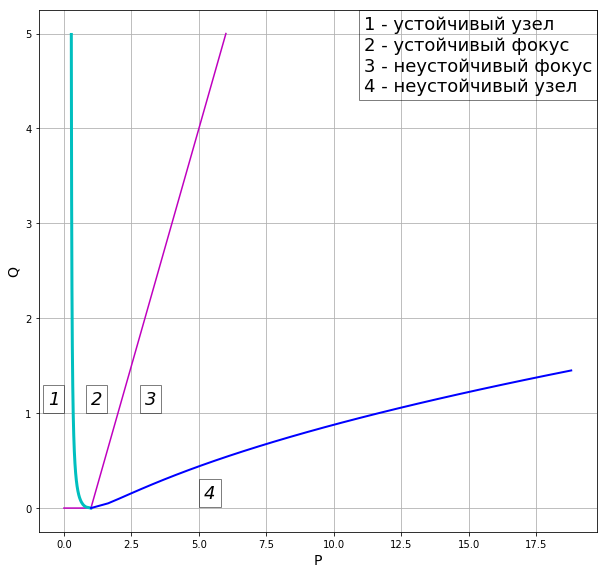
\includegraphics[scale=0.35]{pics/bifurcation_plot}}
\end{figure}
\end{frame}
\begin{frame}
\frametitle{Примеры фазовых портретов}
\begin{figure}[h!]
\vspace{-1em}
\center{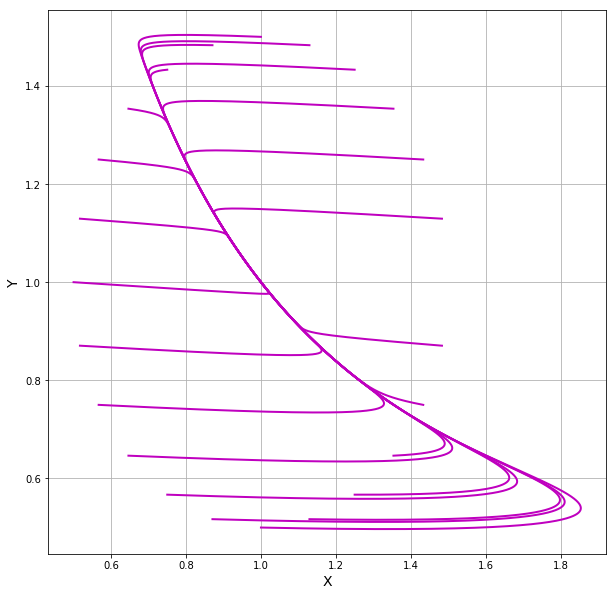
\includegraphics[scale=0.34]{pics/nodeP=005Q=1}}
\vspace{-2em}
\center{Устойчивый узел, $p$=0.05, $q$=1}
\end{figure}
\end{frame}
\begin{frame}
\frametitle{Примеры фазовых портретов}
\begin{figure}[h!]
\vspace{-1em}
\center{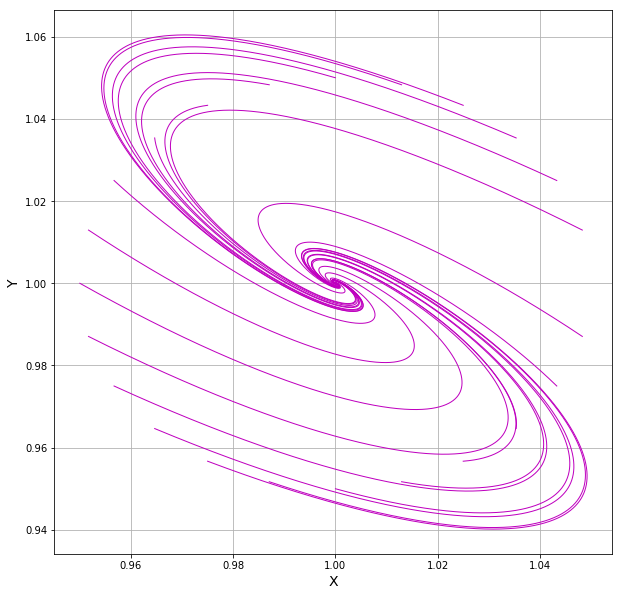
\includegraphics[scale=0.34]{pics/focusP=07Q=1}}
\vspace{-2em}
\center{Устойчивый фокус, $p$=0.7, $q$=1}
\end{figure}
\end{frame}
\begin{frame}
\frametitle{Примеры фазовых портретов}
\begin{figure}[h!]
\vspace{-1em}
\center{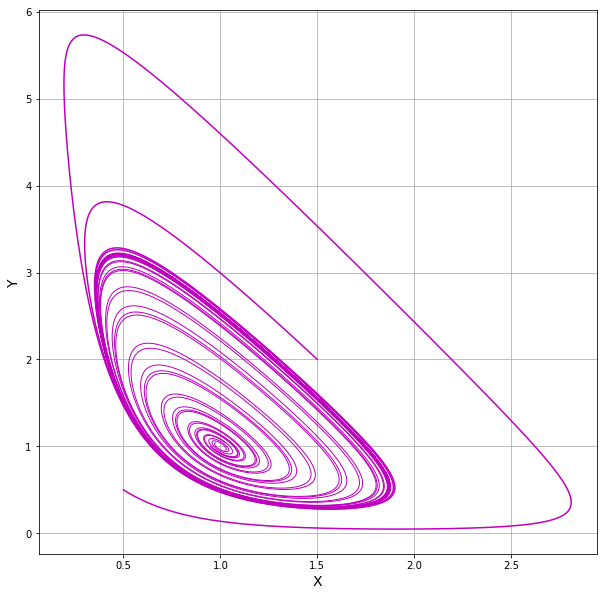
\includegraphics[scale=0.34]{pics/focusP=2_5Q=1}}
\vspace{-2em}
\center{Неустойчивый фокус, $p$=2.5, $q$=1}
\end{figure}
\end{frame}
\begin{frame}
\frametitle{Примеры фазовых портретов}
\begin{figure}[h!]
\vspace{-1em}
\center{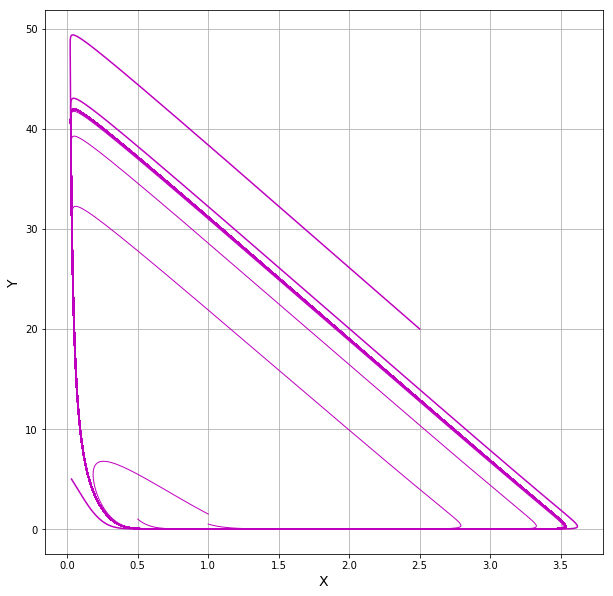
\includegraphics[scale=0.34]{pics/nodeP=12_5Q=1}}
\vspace{-2em}
\center{Неустойчивый узел, $p$=12.5, $q$=1}
\end{figure}
\end{frame}
\begin{frame}
\frametitle{Предельные циклы}
\vspace{3em}
В случаях, когда фазовый портрет системы неустойчив, на фазовой плоскости присутствуют предельные циклы. Их размер и форма изменяются в зависимости от параметров $p$ и $q$, также представляет интерес вопрос об их устойчивости. Предельные циклы могут быть найдены с некоторой наперед заданной точностью 
\end{frame}
\begin{frame}
\frametitle{Пример предельного цикла}
\begin{figure}[h!]
\vspace{-1em}
\center{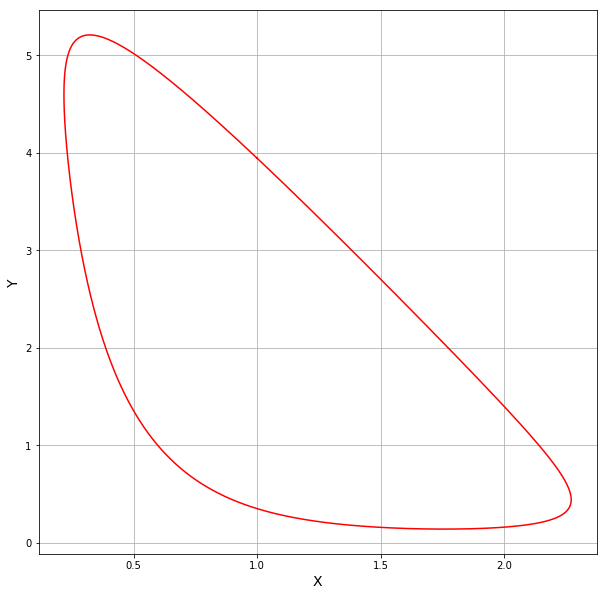
\includegraphics[scale=0.34]{pics/cycp3}}
\vspace{-2em}
\center{$p$=3, $q$=1}
\end{figure}
\end{frame}
\begin{frame}
\frametitle{Пример предельного цикла}
\begin{figure}[h!]
\vspace{-1em}
\center{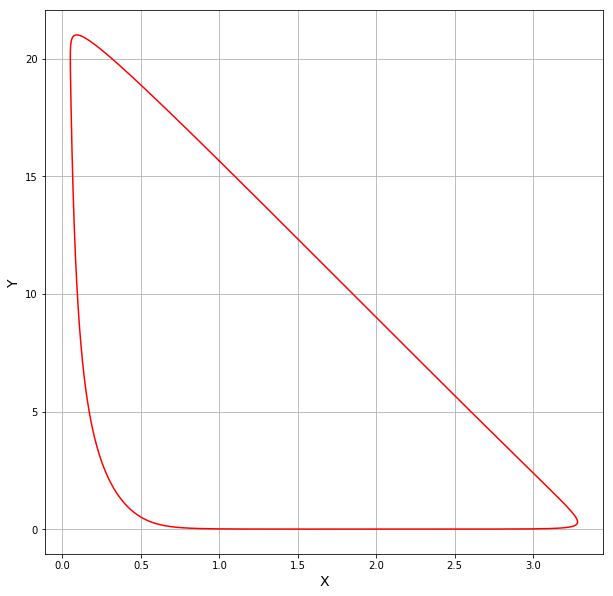
\includegraphics[scale=0.34]{pics/cycp7}}
\vspace{-2em}
\center{$p$=7, $q$=1}
\end{figure}
\end{frame}
\begin{frame}
\frametitle{Пример предельного цикла}
\begin{figure}[h!]
\vspace{-1em}
\center{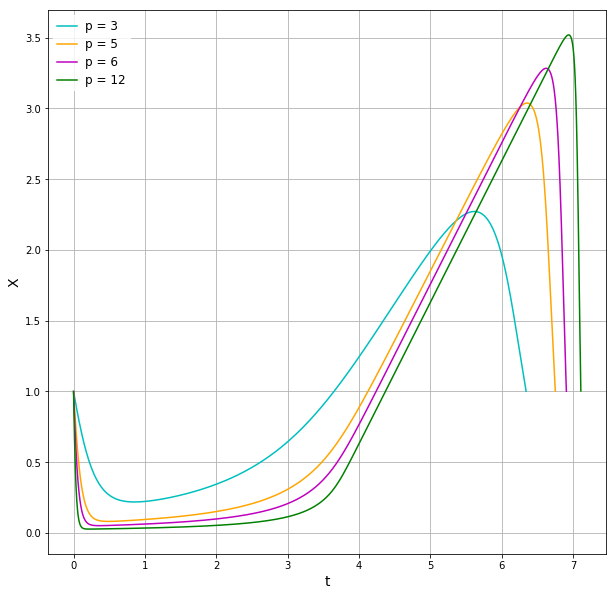
\includegraphics[scale=0.34]{pics/timerowx}}
\vspace{-2em}
\center{Временные ряды для переменной $x$, при $q$=1}
\end{figure}
\end{frame}
\begin{frame}
\frametitle{Пример предельного цикла}
\begin{figure}[h!]
\vspace{-1em}
\center{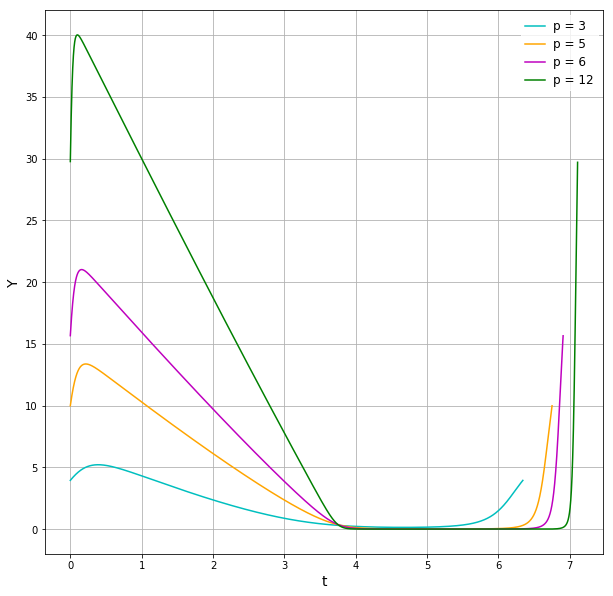
\includegraphics[scale=0.34]{pics/timerowy}}
\vspace{-2em}
\center{Временные ряды для переменной $y$, при $q$=1}
\end{figure}
\end{frame}
\begin{frame}
\frametitle{Устойчивость предельных циклов}
\begin{figure}[h!]
\vspace{-1em}
\center{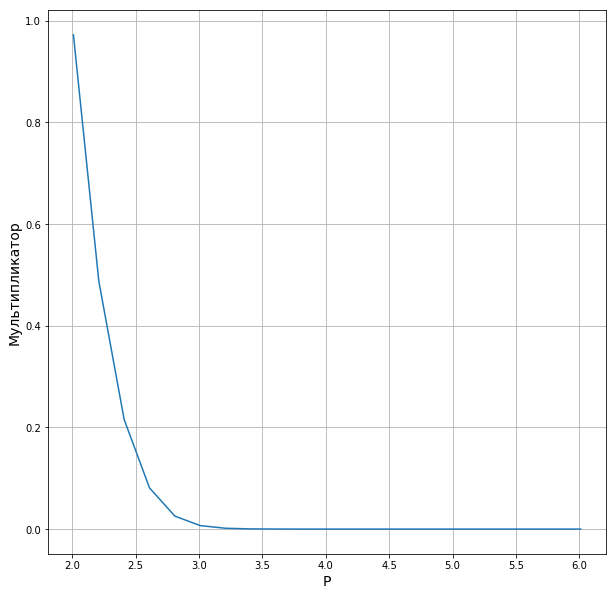
\includegraphics[scale=0.34]{pics/multiplicator}}
\vspace{-2em}
\center{График мультипликатора  $\lambda (p)$}
\end{figure}
\end{frame}
\begin{frame}
\frametitle{Стохастические свойства модели}
\vspace{4em}
Для дальнейшего исследования свойств модели внесем в её поведение случайные возмущения вида $\varepsilon  \sqrt{h} \xi$, где $\xi$ --- нормально распределённая случайная величина, $h$ --- шаг численного метода, $\varepsilon$ --- положительное число, коэффициент, регулирующий интенсивность возмущений.
\end{frame}
\begin{frame}
\frametitle{Возмущения в окрестности устойчивой точки покоя}
\begin{figure}[h!]
\vspace{-1em}
\center{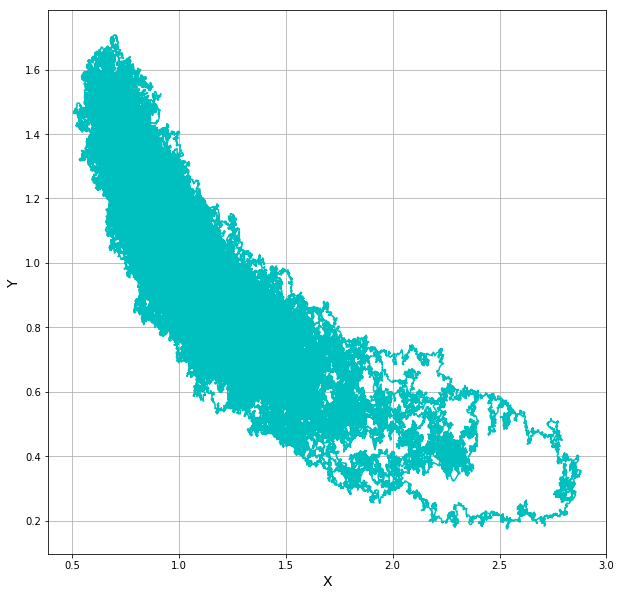
\includegraphics[scale=0.34]{pics/N0_1p0_2q1}}
\vspace{-2em}
\center{Возмущенная траектория $N$=0.1, $p$=0.2, $q$=1}
\end{figure}
\end{frame}
\begin{frame}
\frametitle{Возмущения в окрестности устойчивой точки покоя}
\begin{figure}[h!]
\vspace{-1em}
\center{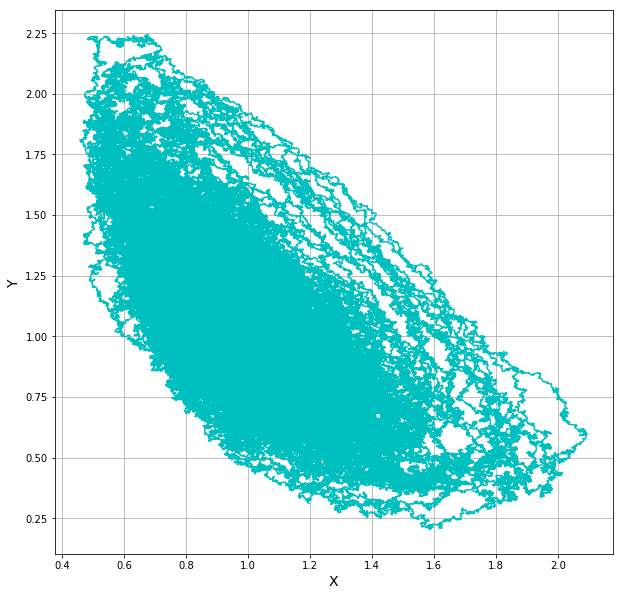
\includegraphics[scale=0.34]{pics/N0_1p1_4q1}}
\vspace{-2em}
\center{Возмущенная траектория $N$=0.1, $p$=1.4, $q$=1}
\end{figure}
\end{frame}
\begin{frame}
\frametitle{Дисперсия возмущенной траектории}
\vspace{4em}
В качестве характеристики поведения возмущённой траектории вблизи устойчивой точки покоя представляет интерес среднеквадратичное отклонение точек траектории от их математического ожидания, которое, заметим, почти совпадает с точкой покоя.
\end{frame}
\begin{frame}
\frametitle{Дисперсия возмущенной траектории}
\begin{figure}[h!]
\vspace{-1em}
\center{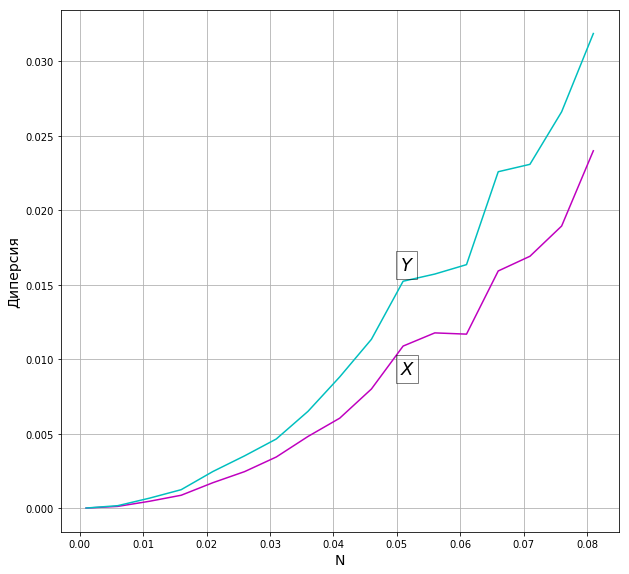
\includegraphics[scale=0.34]{pics/dispN}}
\vspace{-2em}
\center{Зависимость дисперсии от интенсивности шума, $p$=0.2, $q$=1}
\end{figure}
\end{frame}
\begin{frame}
\frametitle{Дисперсия возмущенной траектории}
\begin{figure}[h!]
\vspace{-1em}
\center{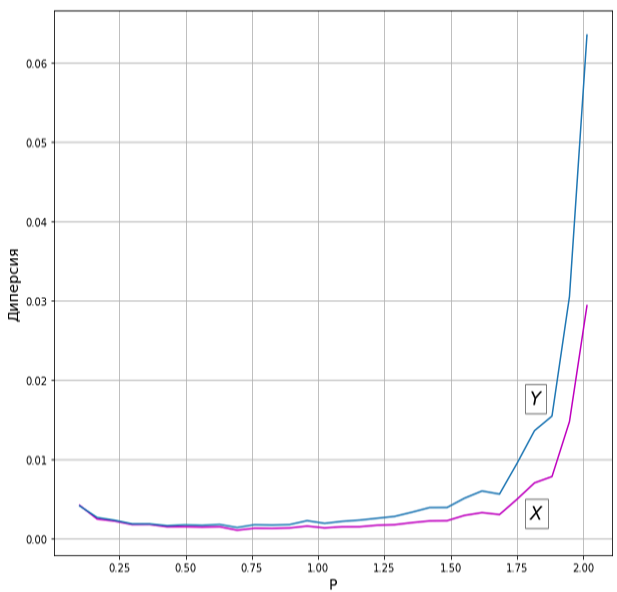
\includegraphics[scale=0.34]{pics/dispP}}
\vspace{-2em}
\center{Зависимость дисперсии от параметра $p$, $N$ = 0.05, $q$~=~1}
\end{figure}
\end{frame}
\begin{frame}
\frametitle{Функция стохастической чувствительности}
\vspace{2.5em}
Функция стохастической чувствительности, далее ФСЧ, позволяет судить о восприимчивости аттрактора системы к случайным возмущениям. ФСЧ точки покоя представляет собой неотрицательное вещественное число, ФСЧ предельного цикла является периодической функцией времени $W(t)$, период которой $T$ совпадает с периодом решения системы, являющегося предельным циклом.
\end{frame}
\begin{frame}
\frametitle{ФСЧ точки покоя}
\vspace{-2.5em}
$$\dot{x} = f(x),$$
$$\dot{x} = f(x)+\varepsilon \sigma (x) \xi (t),$$
$$F W + W F^\mathrm{T} = -S,\, F = \ddfrac{\partial f}{\partial x}(\bar{x}),\, S = GG^\mathrm{T},\, G = \sigma(\bar{x}).$$
\vspace{0.2em}
$$w_{1 2} = (-p^2-p q^2-p q-q^2-2 q-1)/(2 q p (p-q-1))$$
$$w_{1 2} = w_{2 1} = (p^2q+p^2+q^2+2q+1)/(2qp(p-q-1))$$
$$ w_{2 2} = -((q+1)(p^2q+p^2+pq+q+1))/(2qp(p-q-1)).$$
\end{frame}
\begin{frame}
\frametitle{ФСЧ точки покоя}
\begin{figure}[h!]
\vspace{-1em}
\center{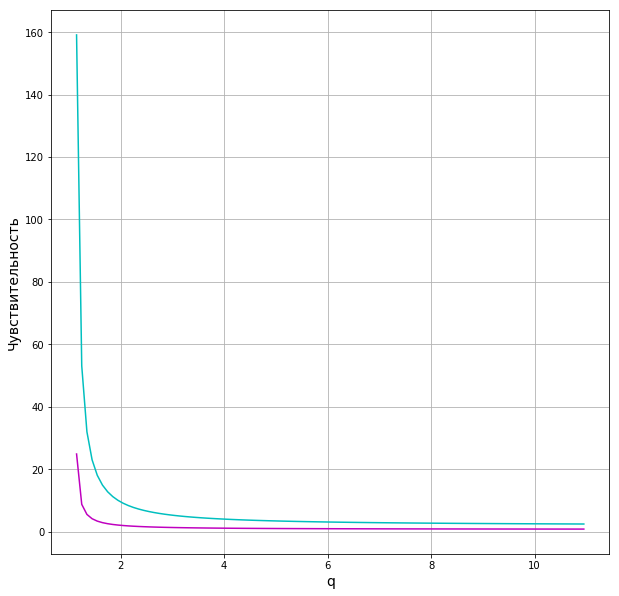
\includegraphics[scale=0.34]{pics/p21nsas}}
\vspace{-2em}
\center{Зависимость ФСЧ от $q$, $p$=2.1}
\end{figure}
\end{frame}
\begin{frame}
\frametitle{ФСЧ предельного цикла}
\vspace{-1em}
Для случая, когда аттрактором является T-периодическое решение системы, задающее предельный цикл $\gamma (t)$, уравнение для $W$ в условиях нашей системы можно записать как:
\vspace{-1em}
$$W(t) = \mu (t)P(t)$$
\vspace{-2.5em}$$\dot\mu = a(t)\mu + b(t),\, \mu(0) = \mu(T)$$
\vspace{-2em}$$a(t) = p^\mathrm{T}(t)(F^\mathrm{T}(t)+ F(t))p(t),\, b(t) = p^\mathrm{T}(t)S(t)p(t),$$
где $p(t)$ - нормализованный нормальный вектор к $f(\gamma(t))$, а $P(t)=pp^\mathrm{T}$.
\end{frame}
\begin{frame}
\frametitle{ФСЧ предельного цикла}
\begin{figure}[h!]
\vspace{-1em}
\center{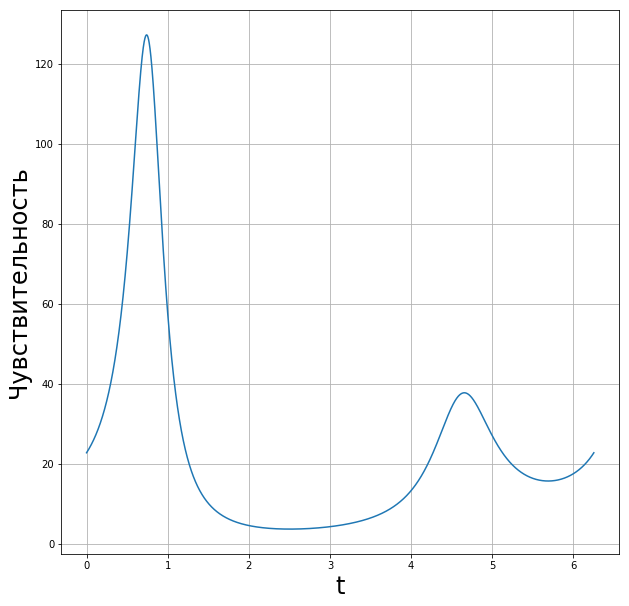
\includegraphics[scale=0.34]{pics/msp2_1q1n0_002}}
\vspace{-2em}
\center{ФСЧ цикла, $p$=2.1, $q$=1, $N$=0.002}
\end{figure}
\end{frame}
\begin{frame}
\frametitle{Доверительный эллипс и доверительная полоса}
\vspace{1em}
Доверительный эллипс строится для устойчивой точки покоя на основе ФСЧ и позволяет ограничить на фазовой плоскости такую её окрестность $U$, что точка с траектории с начальными условиями из $U$ будет принадлежать этой окрестности с заданной наперед вероятностью при данном уровне шума. Доверительная полоса - это аналог доверительного эллипса для случая, когда аттрактором системы выступает устойчивый предельный цикл.
\end{frame}
\begin{frame}
\frametitle{Доверительный эллипс}
\begin{figure}[h!]
\vspace{-1em}
\center{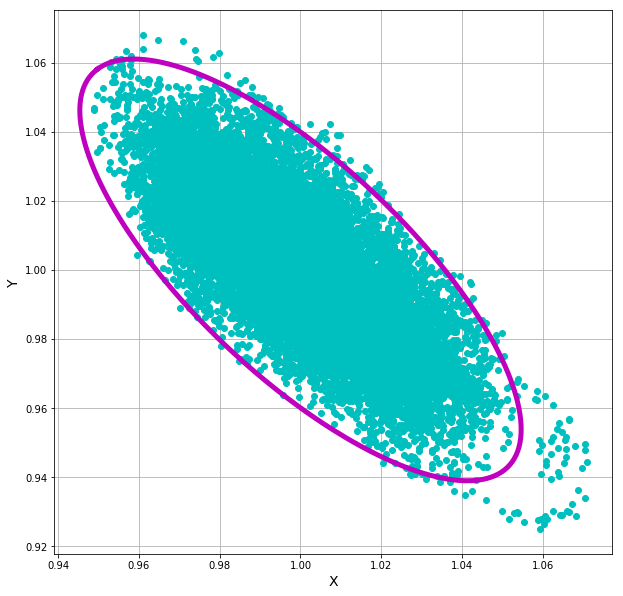
\includegraphics[scale=0.34]{pics/NoisyCurveP0_7Q1}}
\vspace{-2em}
\center{Доверительный эллипс и траектория, $p$=0.7, $q$=1, $N$=0.01}
\end{figure}
\end{frame}
\begin{frame}
\frametitle{Доверительный эллипс}
\begin{figure}[h!]
\vspace{-1em}
\center{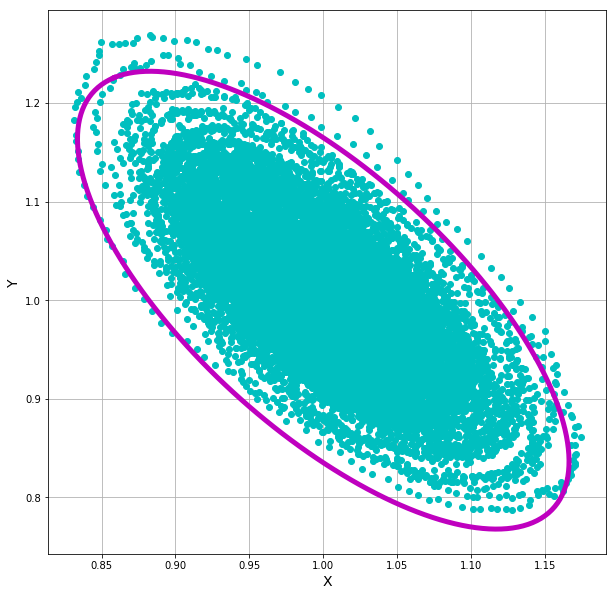
\includegraphics[scale=0.34]{pics/NoisyCurveP1_9Q1}}
\vspace{-2em}
\center{Доверительный эллипс и траектория, $p$=1.9, $q$=1, $N$=0.01}
\end{figure}
\end{frame}
\begin{frame}
\frametitle{Доверительный эллипс}
\begin{figure}[h!]
\vspace{-1em}
\center{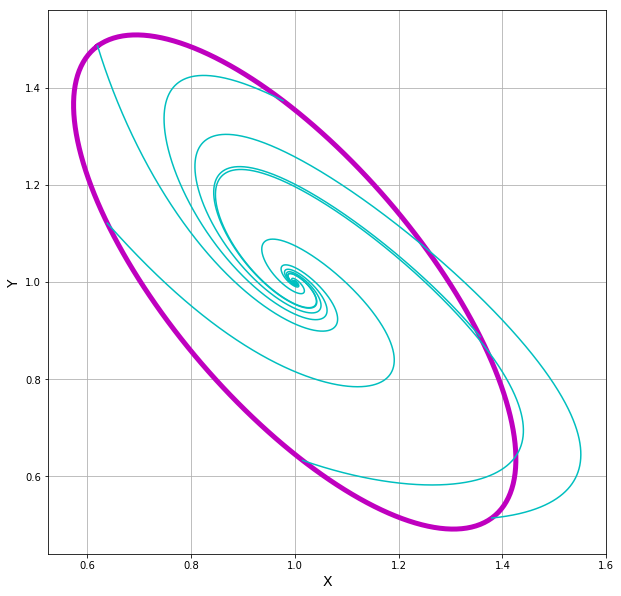
\includegraphics[scale=0.3]{pics/ell075}}
\vspace{-2em}
\center{Доверительный эллипс и детерминированные траектории, $p$=1, $q$=1, $N$=0.075}
\end{figure}
\end{frame}
\begin{frame}
\frametitle{Доверительный эллипс}
\begin{figure}[h!]
\vspace{-1em}
\center{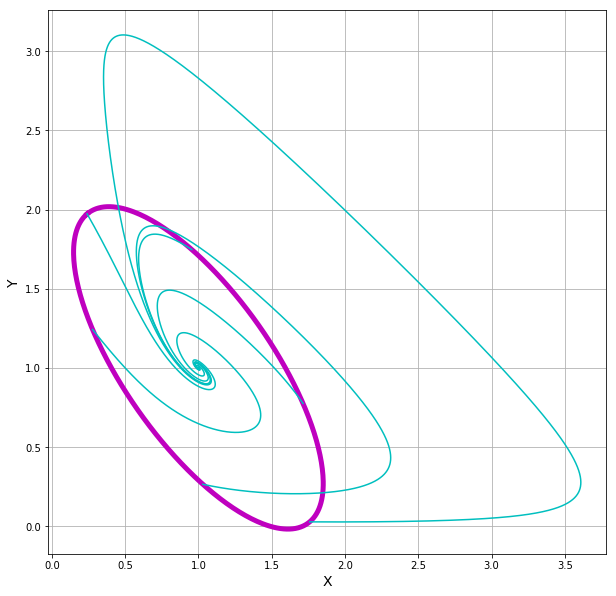
\includegraphics[scale=0.3]{pics/ell015}}
\vspace{-2em}
\center{Доверительный эллипс и детерминированные траектории, $p$=1, $q$=1, $N$=0.15}
\end{figure}
\end{frame}
\begin{frame}
\frametitle{Доверительная полоса}
\begin{figure}[h!]
\vspace{-1em}
\center{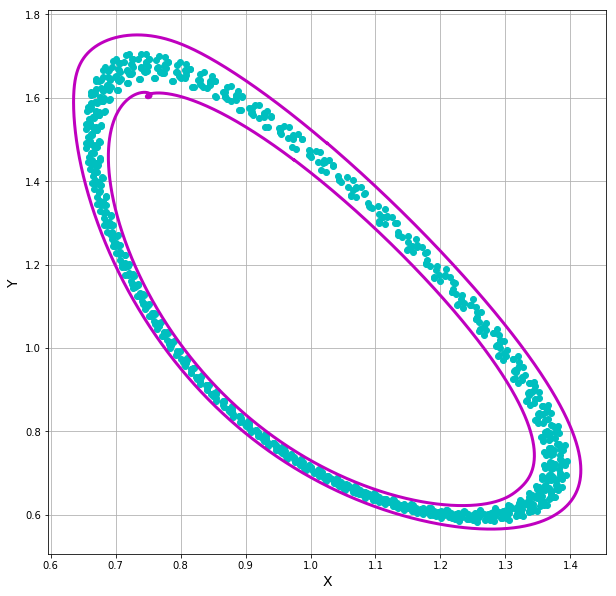
\includegraphics[scale=0.34]{pics/dpp2_1q1}}
\vspace{-2em}
\center{Доверительная полоса и траектория, $p$ = 2.1, $q$ = 1, $N$~=~0.002}
\end{figure}
\end{frame}
\begin{frame}
\frametitle{Индуцированные шумом осцилляции}
\vspace{1em}
При значении параметра $p$=2.1 и $q\in[0.01, 0.12]$ в поведении системы наблюдаются индуцированные шумом осцилляции. При внесении шума порядка 0.002 помимо осцилляций в окрестности детерминированного цикла для данных значениий параметров, наблюдаются осцилляции по большему циклу, причем отношение количества осцилляций по большому циклу к общему числу осцилляций меняется в зависимости от значения параметра $q$, увеличиваясь при его увеличении.
\end{frame}
\begin{frame}
\frametitle{Индуцированные шумом осцилляции}
\begin{figure}[h!]
\vspace{-1em}
\center{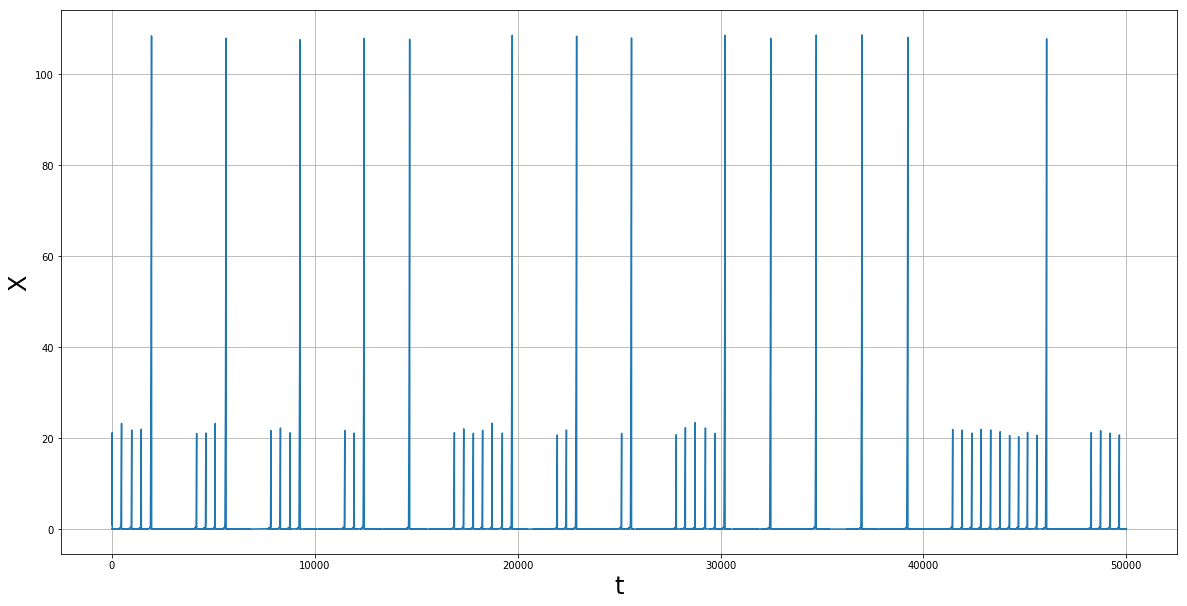
\includegraphics[scale=0.25]{pics/oss05}}
\vspace{-1em}
\center{Временной ряд по переменной $x$, $p$ = 2.1, $q$ = 0.05, $N$~=~0.002}
\end{figure}
\end{frame}
\begin{frame}
\frametitle{Индуцированные шумом осцилляции}
\begin{figure}[h!]
\vspace{-1em}
\center{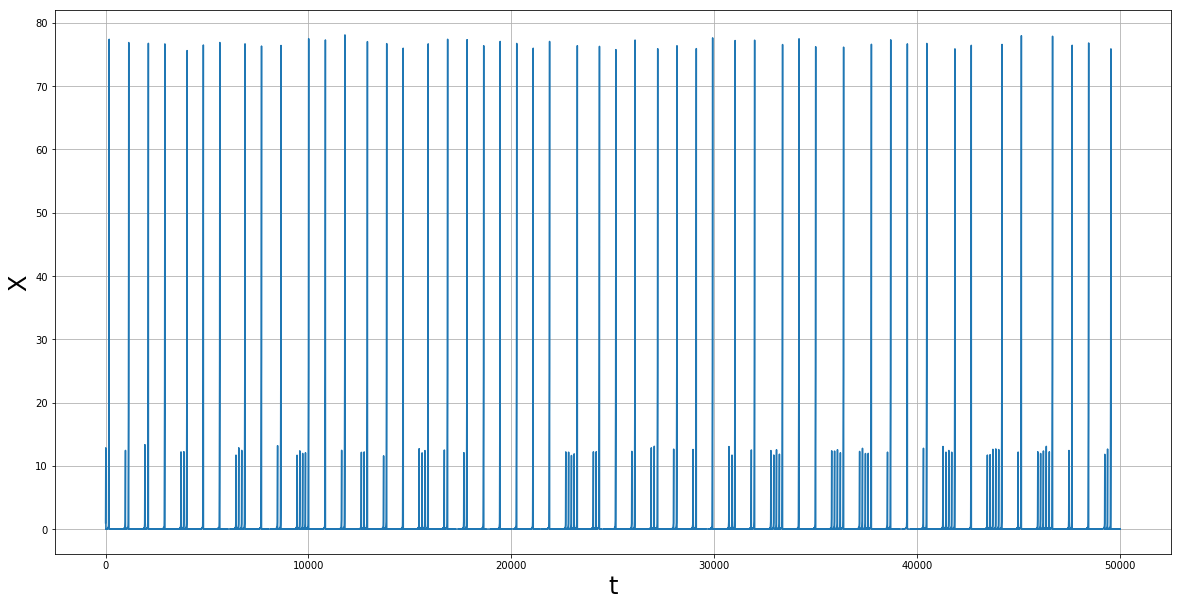
\includegraphics[scale=0.25]{pics/oss01}}
\vspace{-1em}
\center{Временной ряд по переменной $x$, $p$ = 2.1, $q$ = 0.1, $N$~=~0.002}
\end{figure}
\end{frame}
\begin{frame}
\frametitle{Индуцированные шумом осцилляции}
\begin{figure}[h!]
\vspace{-1em}
\center{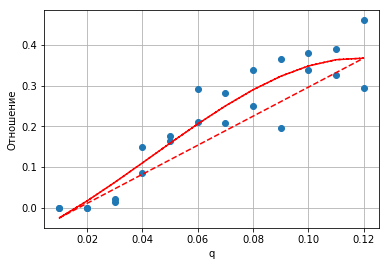
\includegraphics[scale=0.65]{pics/AAAA}}
\vspace{-1em}
\center{Отношение числа больших осцилляций к числу всех осцилляций $p$ = 2.1, $N$~=~0.002}
\end{figure}
\end{frame}
\begin{frame}
\frametitle{Область аномальной стохастической чувствительности}
\vspace{2em}
При значении параметра $q$=0.1 и $p\in[1.1333309, 1.133331]$ наблюдаются большие значения функции стохастической чувствительности и, соответственно, чувствительность к шумам. Так, амплитуды предельных циклов для детерминированных траекторий, построенных при $q$=0.1, $p$=1.1333309 и $q$=0.1, $p$=1.133331 различаются в четыре раза.
\end{frame}
\begin{frame}
\frametitle{Область аномальной стохастической чувствительности}
\begin{figure}[h!]
\vspace{-1em}
\center{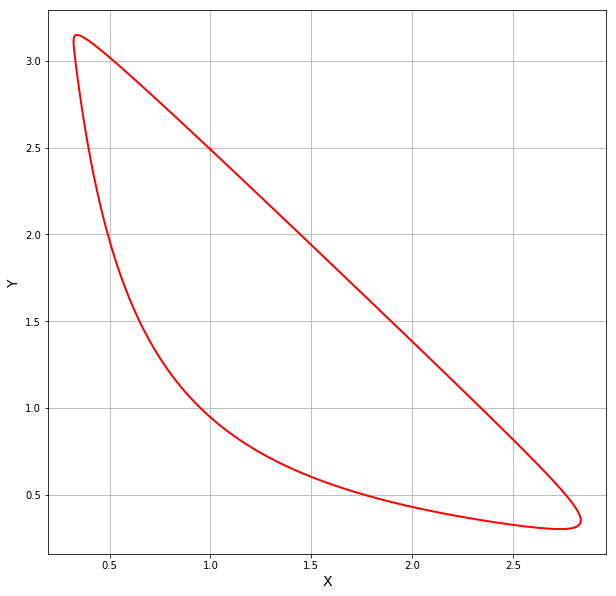
\includegraphics[scale=0.34]{pics/minicyc}}
\vspace{-2em}
\center{Детерминированный цикл $q$=0.1, $p$=1.1333309}
\end{figure}
\end{frame}
\begin{frame}
\frametitle{Область аномальной стохастической чувствительности}
\begin{figure}[h!]
\vspace{-1em}
\center{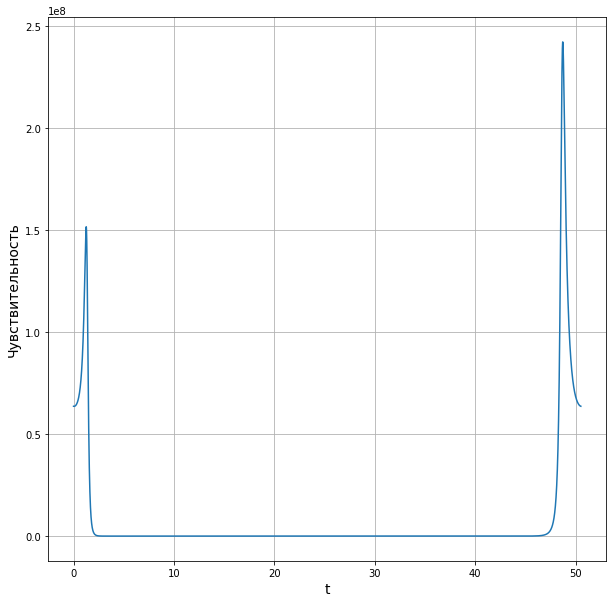
\includegraphics[scale=0.34]{pics/minisens}}
\vspace{-2em}
\center{ФСЧ цикла, $p$=1.1333309, $q$=0.1, $N$=0.00001}
\end{figure}
\end{frame}
\begin{frame}
\frametitle{Область аномальной стохастической чувствительности}
\begin{figure}[h!]
\vspace{-1em}
\center{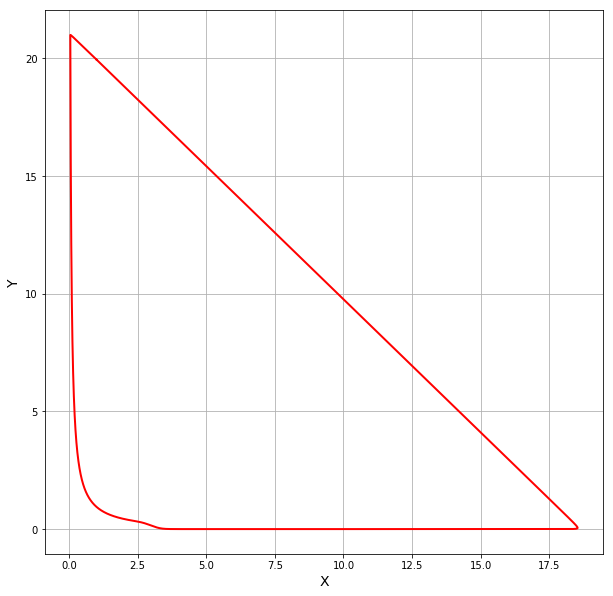
\includegraphics[scale=0.34]{pics/bigcyc}}
\vspace{-2em}
\center{Детерминированный цикл $q$=0.1, $p$=1.133331}
\end{figure}
\end{frame}
\begin{frame}
\frametitle{Область аномальной стохастической чувствительности}
\begin{figure}[h!]
\vspace{-1em}
\center{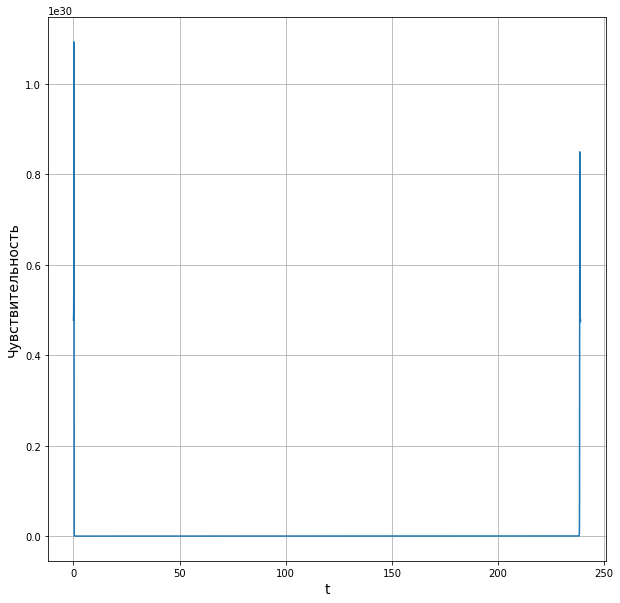
\includegraphics[scale=0.34]{pics/sss}}
\vspace{-2em}
\center{ФСЧ цикла, $p$=1.133331, $q$=0.1, $N$=0.00001}
\end{figure}
\end{frame}
\begin{frame}
\vspace{8em}
\center{\LARGE{Спасибо за внимание!}}
\end{frame}
\end{document}